\chapter{Test Functions}

\section*{Summary}
As indicated in the introduction one must work consistently with smooth ``test functions'' in the theory of distributions. In this chapter we have collected the basic facts that one needs to know about such functions. As an introduction a brief summary of differential calculus is given in \Cref{Section 1.1}. It is written with a reader in mind who has seen the material before but perhaps with different emphasis and different notation. The reader who finds the presentation hard to follow is recommended to study first a more thorough modern treatment of differential calculus in several variables, and experienced readers should proceed directly to \Cref{Section 1.2}. In addition to the basic indispensible facts we have included in Sections \ref{Section 1.3} and \ref{Section 1.4} some more refined constructions which will be useful some time in this book but are not important for the main theme. The reader in a hurry may therefore wish to omit \Cref{Section 1.3} from \Cref{Theorem 1.3.5} on and also \Cref{Theorem 1.4.2}, \Cref{Lemma 1.4.3} and the rest of \Cref{Section 1.4} from \Cref{Theorem 1.4.6} on.

\section{A Review of Differential Calculus}
At first we shall consider functions of a single real variable but permit values in a Banach space. Thus let $I$ be an open interval on the real line $\mathbb{R}$ and let $V$ be a Banach space with norm denoted $\|\cdot \|$. A map $f$ : $I \rightarrow V$ is called differentiable at $x \in I$, with derivative $f'(x) \in V$, if
\begin{equation}
	\label{(1.1.1)}
	\left\| \frac{f(x+h)-f(x)}{h}-f'(x)\right\| \rightarrow 0 \quad \text { when } h \rightarrow 0.
\end{equation}
We can write \eqref{(1.1.1)} in the equivalent form
\begin{equation}
	\label{(1.1.1)'}
	\left\|f(x+h)-f(x)-f'(x) h\right\|=o(|h|) \quad \text{when } h \rightarrow 0.
\end{equation}
If $V=\mathbb{R}^{n}$ and we write $f=\left(f_{1}, \ldots, f_{n}\right)$ then differentiability of $f$ is of course equivalent to differentiability of each component $f_{j}$. For vector
valued functions the mean value theorem must be replaced by the following
\begin{theorem}
	If $f: I \rightarrow V$ is differentiable at every point in $I$, then
	\begin{equation}
		\label{(1.1.2)}
		\|f(y)-f(x)\| \leqq|y-x| \sup \left\{\left\|f'(x+t(y-x))\right\|, 0 \leqq t \leqq 1\right\}; \quad x, y \in I.
	\end{equation}
\end{theorem}
\begin{proof}
	Let $M>\sup \left\{\left\|f'(x+t(y-x))\right\|, 0 \leqq t \leqq 1\right\}$ and set
	\[
		E=\{t ; 0 \leqq t \leqq 1,|| f(x+t(y-x))-f(x) \| \leqq M t|x-y|\}
	\]
	$E$ is closed since $f$ is continuous, and $0 \in E$, so $E$ has a largest element $s$. If $t>s$ and $t-s$ is sufficiently small we have
	\[
		\begin{aligned}
			 & \|f(x+t(y-x))-f(x)\|                                            \\
			 & \quad \leqq\|f(x+t(y-x))-f(x+s(y-x))\| + \| f(x+s(y-x))-f(x) \| \\
			 & \quad \leqq M|(t-s)(y-x)|+M s|y-x|=M t|y-x|
		\end{aligned}
	\]
	Hence $s=1$ which proves the theorem.
\end{proof}
\begin{remark}
	If $f$ is just continuous in $[x, y]$ and differentiable in the interior we obtain \eqref{(1.1.2)} with supremum for $0<t<1$ as a limit of \eqref{(1.1.2)} applied to smaller intervals. If $v \in V$ an application of \eqref{(1.1.2)} to $x \rightarrow f(x)-x v$ gives
	\begin{equation}
		\label{(1.1.2)'}
		\|f(y)-f(x)-v(y-x)\| \leqq|y-x| \sup _{0<t<1}\left\|f'(x+t(y-x))-v\right\|.
	\end{equation}
	which is often more useful, particularly with $v=f'(x)$.
\end{remark}

\begin{cor}
	Let $f$ be continuous in $I$ and differentiable outside a closed subset $F$ where $f=0$. If $x \in F$ and $f'(y) \rightarrow 0$ when $I \setminus F \ni y \rightarrow x$, then $f'(x)$ exists and is equal to $0$.
\end{cor}
\begin{proof}
	If $y \in F$ then $f(y)-f(x)=0$. Otherwise let $z$ be the point in $F \cap[x, y]$ closest to $y$. Then \eqref{(1.1.2)} gives
	\[
		\|f(y)-f(x)\|=\|f(y)-f(z)\| \leqq|y-z| \sup _{0<t<1}\left\|f'(z+t(y-z))\right\|
	\]
	which is $o(|y-x|)$ as $y \rightarrow x$.
\end{proof}

\begin{example}
	If $P$ is a polynomial and $f(x)=P(1 / x) e^{-1 / x}, x>0, f(x)=0, x \leqq 0$, then $f$ is continuous. The derivative for $x \neq 0$ is of the same form with $P(1 / x)$ replaced by $\left(P(1 / x)-P'(1 / x)\right) / x^{2}$ so $f'(0)$ exists and is equal to $0$.
\end{example}

Let $U$ be another Banach space, $X$ an open subset of $U$. If $f$ is a function from $X$ to $V$ we define differentiability by an analogue of \eqref{(1.1.1)}:

\begin{defi}
	$f$ is called differentiable at $x \in X$ if there is an element $f'(x) \in L(U, V)$ such that
	\begin{equation}
		\label{(1.1.1)''}
		\left\|f(x+h)-f(x)-f'(x) h\right\|=o(\|h\|), \quad h \rightarrow 0
	\end{equation}
	Here $L(U, V)$ is the space of continuous linear transformations from $U$ to $V$, which is a Banach space with the norm
	\[
		\|T\|=\sup _{\|x\|<1}\|T x\|, \quad T \in L(U, V)
	\]
	By $C^{1}(X, V)$ we denote the set of continuously differentiable functions from $X$ to $V$, that is, the set of functions $f$ which are differentiable at every point and for which $X \ni x \rightarrow f'(x) \in L(U, V)$ is continuous.
\end{defi}

If $f$ is just differentiable at every point on the line segment $[x, y]=\{x+t(y-x) ; 0 \leqq t \leqq 1\}$ then \eqref{(1.1.2)} gives for every $T \in L(U, V)$
\begin{equation}
	\label{(1.1.2)''}
	\|f(y)-f(x)-T(y-x)\| \leqq\|y-x\| \sup _{0<t<1}\left\|f'(x+t(y-x))-T\right\|
\end{equation}
for $f(x+t(y-x))-T t(y-x)$ is differentiable in $t$ on $[0,1]$ with derivative
\[
	f'(x+t(y-x))(y-x)-T(y-x) .
\]

\begin{theorem}
	If $f_{j} \in C^{1}(X, V)$ and $f_{j} \rightarrow f, f_{j}' \rightarrow g$ locally uniformly in $X$, then $f \in C^{1}(X, V)$ and $f'=g$.
\end{theorem}
\begin{proof}
	If we apply \eqref{(1.1.2)''} to $f_{j}$ with $T=f_{j}'(x)$ we obtain when $j \rightarrow \infty$
	\[
		\|f(y)-f(x)-g(x)(y-x)\| \leqq\|y-x\| \sup _{0<t<1}\|g(x+t(y-x))-g(x)\|
	\]
	which proves that $f$ is differentiable at $x$ with $f'(x)=g(x)$. Since $g$ is continuous this proves the theorem.
\end{proof}
\begin{theorem}
	If $f$ and $g$ are continuous functions in $X$ with values in $V$ and $L(U, V)$ respectively, and $t \rightarrow f(x+t y)$ is for all $x, y \in U$ differentiable with respect to $t$ with derivative $g(x+t y) y$ when $x+t y \in X$, then $f \in C^{1}$ and $f'=g$. It suffices to make the hypothesis for all $y$ in a set $Y\subset U$ with closed linear hull equal to $U$.
\end{theorem}
\begin{proof}
	\eqref{(1.1.2)'} gives for small $\|y\|$
	\[
		\|f(x+y)-f(x)-g(x) y\| \leqq\|y\| \sup _{0<t<1}\|g(x+t y)-g(x)\|
	\]
	which proves the first statement. To prove the second one it suffices to show that the set of all $y$ for which the hypothesis holds is linear and closed. This follows from \eqref{(1.1.2)'}; the details are left for the reader.
\end{proof}

If $f$ is a linear map $U \rightarrow V$ then $f$ is of course differentiable and $f'(x)=f$ for every $x$. More generally, let $U_{1}, \ldots, U_{k}$ be Banach spaces and $L\left(U_{1}, \ldots, U_{k} ; V\right)$ the space of multilinear maps
\[
	U_{1} \times \ldots \times U_{k} \ni\left(x_{1}, \ldots, x_{k}\right) \rightarrow f\left(x_{1}, \ldots, x_{k}\right) \in V
\]
which are continuous, that is,
\[
	\|f\|=\sup _{\left\|x_{j}\right\|<1}\left\|f\left(x_{1}, \ldots, x_{k}\right)\right\|<\infty
\]
With this norm $L\left(U_{1}, \ldots, U_{k} ; V\right)$ is a Banach space. The map
\[
	U_{1} \oplus \ldots \oplus U_{k} \ni\left(x_{1}, \ldots, x_{k}\right) \rightarrow f\left(x_{1}, \ldots, x_{k}\right) \in V
\]
is differentiable for every $\left(x_{1}, \ldots, x_{k}\right)$, and the differential is
\[
	\begin{aligned}
		 & U_{1} \oplus \ldots \oplus U_{k} \ni\left(y_{1}, \ldots, y_{k}\right) \rightarrow f\left(y_{1}, x_{2}, \ldots, x_{k}\right) \\
		 & \quad+f\left(x_{1}, y_{2}, \ldots, x_{k}\right)+\ldots+f\left(x_{1}, x_{2}, \ldots, x_{k-1}, y_{k}\right)
	\end{aligned}
\]

Another important example of a $C^{1}$ map is for two Banach spaces $U$ and $V$ the map $f$ taking an invertible element $T \in L(U, V)$ to its inverse $T^{-1} \in L(V, U)$. That $T^{-1}$ is an inverse means that
\[
	T T^{-1}=\mathrm{id}_{V}, \quad T^{-1} T=\mathrm{id}_{U} .
\]
If $S \in L(U, V)$ we have $(T+S) T^{-1}=\mathrm{id}_{V}+S T^{-1}$ so if $\|S\|\left\|T^{-1}\right\|<1$ a right inverse of $T+S$ is given by
\[
	T^{-1}\left(\mathrm{id}_{V}+S T^{-1}\right)^{-1}=\sum_{0}^{\infty} T^{-1}\left(-S T^{-1}\right)^{k}
\]
In the same way we see that it is a left inverse. Thus $f(T)=T^{-1}$ is defined in an open set and
\[
	\left\|f(T+S)-f(T)+T^{-1} S T^{-1}\right\| \leqq\frac{\left\|T^{-1}\right\|^{3}\|S\|^{2}}{1-\|S\|\left\|T^{-1}\right\|}
\]
so $f$ is differentiable at $T$ and $f'(T) S=-T^{-1} S T^{-1}$. Thus $f$ is continuous so $f'$ is continuous.

Next we shall discuss composite functions. Let $X$ as before be an open subset of the Banach space $U, f$ a map from $X$ to a Banach space $V$ with range contained in an open set $Y$ where another map $g$ to a third Banach space $W$ is defined. If $f$ is differentiable at $x$ and $g$ is differentiable at $y=f(x)$ then $h=g \circ f$ is differentiable at $x$ and
\begin{equation}
    \label{(1.1.3)}
    h'(x)=g'(y) f '(x) \quad\text{(the chain rule).}
\end{equation}
The proof is obvious. From \eqref{(1.1.3)} it follows that $h \in C^{1}$ if $g \in C^{1}$ and $f \in C^{1}$.

The differential $f'$ may be viewed as a map
\[
	X \times U \ni(x, t) \xrightarrow{f'}\left(f(x), f'(x) t\right) \in Y \times V
\]
which is linear in the second component which should be thought of as a tangent direction. Then the chain rule says that given a commutative diagram
\[
    \begin{tikzcd}
    {}&\quad\arrow[rd,"g"]&{}\\
    \quad\arrow[ur,"f"]\arrow[rr,"h"']&{}&\quad
    \end{tikzcd}
\]
% \begin{center}
% 	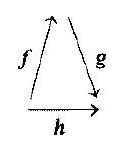
\includegraphics[max width=\textwidth]{2024_02_17_0c416db476dd617ef477g-004(1)}
% \end{center}
with $f, g \in C^{1}$ we obtain $h \in C^{1}$ and another commutative diagram
\[
    \begin{tikzcd}
    {}&\quad\arrow[rd,"g'"]&{}\\
    \quad\arrow[ur,"f'"]\arrow[rr,"h'"']&{}&\quad
    \end{tikzcd}
\]
% \begin{center}
% 	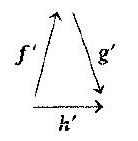
\includegraphics[max width=\textwidth]{2024_02_17_0c416db476dd617ef477g-004}
% \end{center}
Instead of the notation $f'$ one often writes $d f$, particularly when $f$ is real valued. If $f$ is defined in an open set in $\mathbb{R}^{n}$ and we write $t=\sum t_{j} e_{j}$ where $e_{j}$ is the $j^{\text {th }}$ unit vector, then
\[
	(d f)(t)=(d f)\left(\sum t_{j} e_{j}\right)=\sum t_{j} d f\left(e_{j}\right)=\sum \partial f / \partial x_{j} t_{j}
\]
But $t_{j}=\left(d x_{j}\right)(t)$ so we can write this equation in the form
\[
	d f=\sum \frac{\partial f }{\partial x_{j}} d x_{j}
\]
By the chain rule this formula remains valid if $x_{j}$ are in fact functions of $z \in Z$ and both $f$ and $x_{j}$ are regarded as functions on $Z$ so that both sides are linear functions there. This is called the invariance of the differential.

Next we prove the inverse function theorem which shows that differential calculus does accomplish its goal of reducing the study of fairly general equations to linear ones.
\begin{theorem}
    Let $X$ be open in $U$ and $f \in C^{1}(X, V)$, and let $x_{0} \in X$, $f(x_0)=y_{0}$. For the existence of $g \in C^{1}(Y, U)$, where $Y$ is a neighborhood of $y_{0}$, such that a) $f \circ g=$ identity near $y_{0}$ or b) $g \circ f=$ identity near $x_{0}$ or c) $f \circ g=$ identity near $y_{0}$ and $g \circ f=$ identity near $x_{0}$, it is necessary and sufficient that there is a linear map $A \in L(V, U)$ such that respectively
\begin{enumerate}[label=\upshape\alph*)$'$]
    \item\label{thm:1.1.7:label:a} $f'(x_0) A=\mathrm{id}_{V}$
\item\label{thm:1.1.7:label:b} $A f'(x_0)=\mathrm{id}_{U}$
\item\label{thm:1.1.7:label:c} $f'(x_0) A=\mathrm{id}_{V}, A f'(x_0)=\mathrm{id}_{U}$.
\end{enumerate}

The condition c) is equivalent to bijectivity of $f'(x_{0})$ and it implies that $g$ is uniquely determined near $y_{0}$. If $V(U)$ is finite dimensional then \ref{thm:1.1.7:label:a}(\ref{thm:1.1.7:label:b}) is equivalent to surjectivity (injectivity) of $f'(x_{0})$.
\end{theorem}

\begin{proof}
    The necessity is an immediate consequence of the chain rule \eqref{(1.1.3)}. In the proof of the sufficiency we first observe that if $f \circ g_{1}=\mathrm{id}$ near $y_{0}$ and $g_{2} \circ f=\mathrm{id}$ near $x_{0}$ then $g_{1}=g_{2} \circ f \circ g_{1}=g_{2}$ near $y_{0}$ which proves uniqueness in case c) and reduces the proof to existence in cases a) and b). If we replace $f$ by $f \circ A$ resp. $A \circ f$ we see that it suffices to study the case where $U=V$ and $f'(x_0)=$ id. Choose $\delta>0$ so that
\[
	\left\|f'(x)-\mathrm{id}\right\|<\frac{1}{2} \quad \text { when } \quad\left\|x-x_{0}\right\| \leqq \delta.
\]
For $\left\|x_{j}-x_{0}\right\| \leqq \delta, j=1,2$, we have by \eqref{(1.1.2)''}
\begin{equation}
    \label{(1.1.4)}
	\left\|f\left(x_{1}\right)-f\left(x_{2}\right)-\left(x_{1}-x_{2}\right)\right\| \leqq \frac{\left\|x_{1}-x_{2}\right\|}{2}
\end{equation}
Hence $f$ is injective in $\left\{x ;\left\|x-x_{0}\right\| \leqq \delta\right\}$. To solve the equation $f(x)=y$ when $\left\|y-y_{0}\right\|<\delta / 2$ we set
\begin{equation}
    \label{(1.1.5)}
	x_{k}=x_{k-1}+y-f\left(x_{k-1}\right), \quad k=1,2, \ldots
\end{equation}
as long as this leads to points with $\left\|x_{k}-x_{0}\right\|<\delta$. We have
\[
	\left\|x_{1}-x_{0}\right\|=\left\|y-y_{0}\right\|<\frac{\delta}{2}
\]
If $k>1$ and $\left\|x_{j}-x_{0}\right\|<\delta$ when $j<k$ then
\[
	\begin{aligned}
		\left\|x_{k}-x_{k-1}\right\| & =\left\|x_{k-1}-f\left(x_{k-1}\right)-\left(x_{k-2}-f\left(x_{k-2}\right)\right)\right\| \\
		                             & \leqq \frac{\left\|x_{k-1}-x_{k-2}\right\|}{2} < \frac\delta{2^{k}}
	\end{aligned}
\]
by \eqref{(1.1.4)}. Hence
\[
	\left\|x_{k}-x_{0}\right\|<\delta \sum_{1}^{k} 2^{-j}<\delta
\]
so $x_{k}$ is defined for all $k$ and is a Cauchy sequence. For the limit $x$ we have $\left\|x-x_{0}\right\|<\delta$, and when $k \rightarrow \infty$ we obtain $f(x)=y$ from \eqref{(1.1.5)}.

To prove that the inverse $g(y)=x$, which is now defined when $\left\|y-y_{0}\right\|<\delta / 2$, belongs to $C^{1}$ we set
\[
	g(y)=x, \quad g(y+k)=x+h
\]
This means that $f(x+h)=y+k$ and that $f(x)=y$. Hence
\[
	k=f(x+h)-f(x)=f'(x) h+o(\|h\|)
\]
In view of \eqref{(1.1.4)} we have $\|k-h\|<\|h / 2\|$, hence $\|h\| / 2<\|k\|<2\|h\|$. Since $\left\|f'(x)^{-1}\right\|<2$ we obtain
\[
	h=f'(x)^{-1} k+o(\|k\|)
\]
which proves that $g$ is differentiable and that $g'(y)=f'(g(y))^{-1}$, which is a continuous function of $y$.
\end{proof}

We shall now define differentials of higher order and the space $C^{k}(X, V)$ where as before $X$ is an open subset of the Banach space $U$ but $k$ is now an integer $>1$. This is done by induction so $f \in C^{k}(X, V)$ if $f \in C^{1}(X, V)$ and $f' \in C^{k-1}(X, L(U, V))$. The differential $f''$ of $f'$ is called the second differential of $f$, and so on,
\[
	f^{(k)} \in C( X, L( U, L( U, \ldots, L(U, V) ) ) )
\]
The vector space $L(U, L(U, \ldots, L(U, V)))$ is isomorphic as a Banach space to the space $L(U, \ldots, U ; V)=L^{k}(U, V)$ of $k$-linear maps from $U$ to V. In fact, we always have
\[
	L\left(U, L\left(U_{1}, \ldots, U_{j} ; V\right)\right)=L\left(U, U_{1}, \ldots, U_{j} ; V\right)
\]
for if $f$ is an element in the space on the left and the assertion is known when $j$ is replaced by $j-1$, then
\[
	U \times U_{1} \times \ldots \times U_{j} \ni\left(x, x_{1}, \ldots, x_{j}\right) \rightarrow f(x)\left(x_{1}, \ldots, x_{j}\right) \in V
\]
is an element in the space on the right, and all its elements can be so obtained. The correspondence is obviously linear and norm preserving.

By $L_{s}^{k}(U, V)$ we shall denote the space of symmetric $k$ linear forms from $U$ to $V$, that is, forms such that the value at $\left(x_{1}, \ldots, x_{k}\right)$ is not changed by a permutation of $x_{1}, \ldots, x_{k}$.

\begin{theorem}
    If $f \in C^{k}$ then $f^{(k)}$ is a symmetric multilinear form, that is, the order of differentiation is not essential.
\end{theorem}
\begin{proof}
    Set $\Delta_{y} F(x)=F(x+y)-F(x)$. By repeated use of \eqref{(1.1.2)''} we obtain if $L$ is a multilinear form
\[
	\begin{aligned}
		 & \left\|\Delta_{y_{k}} \ldots \Delta_{y_{1}} f(x)-L(y_{1}, \ldots, y_{k})\right\|                                                              \\
		 & \quad \leqq \sup _{0<i<1}\left\|\Delta_{y_{k-1}} \ldots \Delta_{y_{1}} f'(x+t y_{k}) y_{k}-L(y_{1}, \ldots, y_{k})\right\| \\
		 & \quad \leqq \sup _{0<t_{j}<1}\left\|f^{(k)}\left(x+\sum_{1}^{k} t_{j} y_{j} ; y_{1}, \ldots, y_{k}\right)-L(y_{1}, \ldots, y_{k})\right\|
	\end{aligned}
\]
If we choose $L=f^{(k)}(x)$ it follows that
\begin{equation}
    \label{(1.1.6)}
    \left\|\Delta_{y_{k}} \ldots \Delta_{y_{1}} f(x)-f^{(k)}(x ; y_{1}, \ldots, y_{k})\right\|=o\left(\left\|y_{1}\right\| \ldots\left\|y_{k}\right\|\right)
\end{equation}
This determines $f^{(k)}$ completely of course, and since $\Delta_{y_k} \ldots \Delta_{y_{1}} f(x)$ does not depend on the order of the differences it follows that $f^{(k)}(x)$ is symmetric.
\end{proof}

From \eqref{(1.1.3)} it follows at once by induction that $h=g \circ f \in C^{k}$ if $f$, $g \in C^{k}$, for if this is proved for smaller values of $k$ we have $g' \circ f \in C^{k-1}$

and $f' \in C^{k-1}$, and the composition of linear maps
\[
	L(V, W) \times L(U, V) \rightarrow L(U, W)
\]
is continuous, hence infinitely differentiable. The inverse function theorem (\Cref{Theorem 1.1.7}) also remains valid with $C^{1}$ replaced by $C^{k}$ throughout. In fact, the map
\[
	L(U, V) \ni T \rightarrow T^{-1} \in L(V, U)
\]
is in $C^{k}$ where it is defined, with $k^{\text {th}}$ differential
\[
	\left(S_{1}, \ldots, S_{k}\right) \rightarrow(-1)^{k} \sum T^{-1} S_{i_{1}} T^{-1} S_{i_{2}} T^{-1} \ldots S_{i_{k}} T^{-1}
\]
summed over all permutations of $1, \ldots, k$. In the proof of \Cref{Theorem 1.1.7} we therefore obtain inductively that $g \in C^{k}$ if $f \in C^{k}$, by using that $g'(y)=f'(g(y))^{-1}$.

If $f \in C^{k}$ in a neighborhood of the line segment $[x, x+y]$ then we have Taylor's formula
\begin{align}
    \label{(1.1.7)}
	f(x+y)= & \sum_{0}^{k-1} \frac{f^{(j)}(x ; y, \ldots, y)}{j !}     \\
	        & + \frac{1}{(k-1) !}\int_{0}^{1} f^{(k)}(x+t y ; y, \ldots, y)(1-t)^{k-1} d t
\end{align}
This follows inductively by partial integration since
\[
	\frac{d}{d t} f^{(k-1)}(x+t y ; y, \ldots, y)=f^{(k)}(x+t y ; y, \ldots, y)
\]
In particular we obtain
\begin{equation}
    \label{(1.1.8)}
	\left\|f(x+y)-\sum_{0}^{k} \frac{f^{(j)}(x ; y, \ldots, y)}{j!}\right\|=o\left(\|y\|^{k}\right) \quad \text { as } y \rightarrow 0 .
\end{equation}

Let us now assume that $f$ is defined in an open set $X \subset \mathbb{R}^{n}$. It follows from \Cref{Theorem 1.1.6} that $f \in C^{k}$ if and only if all the partial derivatives
\[
	\frac{\partial}{\partial x_{i_{1}}} \cdots \frac{\partial f}{\partial x_{i_{j}}}
\]
of order $j \leqq k$ are defined and continuous. By \Cref{Theorem 1.1.8} we know that the order of differentiation does not matter. With the notation $\partial_{j}=\partial / \partial x_{j}$ we can therefore write these partial derivatives in the form
\[
	\partial_{1}^{\alpha_{1}} \ldots \partial_{n}^{\alpha_{n}} f=\partial^{\alpha} f
\]
where $\alpha=\left(\alpha_{1}, \ldots, \alpha_{n}\right)$ is a multi-index, that is, an $n$-tuple of non-negative integers, and $\partial^{\alpha}=\partial_{1}^{\alpha_{1}} \ldots \partial_{n}^{\alpha_{n}}$. We set $|\alpha|=\sum \alpha_{j}$, which is the order of differentiation. Note that where $\alpha !=\alpha_{1} ! \ldots \alpha_{n} !$ and $y^{\alpha}=y_{1}^{\alpha_{1}} \ldots y_{n}^{\alpha_{n}}$. Hence Taylor's formula can be written
	\begin{align}
        \label{(1.1.7)'}
		f(x+y)= & \sum_{|\alpha|<k} \frac{\partial^{\alpha} f(x) y^{\alpha}}{\alpha !}                                    \\
		        & +k \int_{0}^{1}(1-t)^{k-1} \sum_{|\alpha|=k} \frac{\partial^{\alpha} f(x+t y) y^{\alpha}}{\alpha !} d t
	\end{align}
The following application is often useful:
\begin{theorem}
    If $f \in C^{k}(B)$ where $B=\left\{x \in \mathbb{R}^{n},|x|<R\right\}$ and $k \geqq 1$, then $f(x)-f(0)=\sum x_{j} f_{j}(x)$ where $f_{j} \in C^{k-1}(B), \partial^{\alpha} f_{j}(0)=\partial^{\alpha} \partial_{j} f(0) /(1+|\alpha|)$, and
\begin{equation}
    \label{(1.1.9)}
	\sup _{B}\left|\partial^{\alpha} f_{j}\right| \leqq \sup _{B}\left|\partial^{\alpha} \partial_{j} f\right|, \quad|\alpha|<k . 
\end{equation}
\end{theorem}
\begin{proof}
    Using \eqref{(1.1.7)'} with $k=1$ we can take
\[
	f_{j}(x)=\int_{0}^{1}\left(\partial_{j} f\right)(t x) d t
\]
and $f_{j} \in C^{k-1}$ since the integrand is in $C^{k-1}$. The estimate (1.1.9) is obvious.

Any linear differential operator
\[
	P=\sum_{|\alpha| \leqq m} a_{\alpha}(x) \partial^{\alpha}
\]
can be written in the form $P(x, \partial)$ where
\[
	P(x, \xi)=\sum_{|\alpha| \leqq m} a_{\alpha}(x) \xi^{\alpha}
\]
is a polynomial in $\xi \in \mathbb{R}^{n}$. By convention coefficients are put to the left of differentiations. Note that
\[
	P(x, \xi)=e^{-\langle x, \xi\rangle} P e^{\langle x, \xi\rangle}
\]
Leibniz' formula for the differentiation of a product takes the form
\begin{equation}
    \label{(1.1.10)}
	P(x, \partial)(u v)=\sum\left(P^{(\alpha)}(x, \partial) u\right) \frac{\partial^{\alpha} v}{\alpha !}
\end{equation}
where $P^{(\alpha)}(x, \xi)=\partial_{\xi}^{\alpha} P(x, \xi)$. Indeed, $u \rightarrow P(x, \partial)(u v)$ is a differential operator for fixed $v$, and
\[
	e^{-\langle x, \xi\rangle} P(x, \partial)\left(e^{\langle x, \xi\rangle} v\right)=P(x, \xi+\partial) v=\sum \frac{P^{(\alpha)}(x, \xi) \partial^{\alpha} v}{\alpha !}
\]
by Taylor's formula. We shall refer to \eqref{(1.1.10)} as Leibniz' formula.
\end{proof}

\section{Existence of Test Functions}
For an open set $X$ in $\mathbb{R}^{n}$ we shall denote by $C^{k}(X)$ the space of $k$ times continuously differentiable complex valued functions in $X$ if $k$ is a non-negative integer, and we set
\[
	C^{\infty}(X)=\bigcap C^{k}(X)
\]
with intersection taken for all finite $k$. In the introduction we have seen the need for functions of the following kind:
\begin{defi}
    By $C_{0}^{k}(X)$ we denote the space of all $u \in C^{k}(X)$ with compact support. The elements of $C_{0}^{\infty}(X)$ are called test functions.
\end{defi}
\begin{defi}
    If $u \in C(X)$ then the support of $u$, written $\operatorname{supp} u$, is the closure in $X$ of the set $\{x \in X ; u(x) \neq 0\}$, that is, $\operatorname{supp} u$ is the smallest closed subset of $X$ such that $u=0$ in $X \setminus \operatorname{supp} u$.
\end{defi}

If the definition of a function $u \in C_{0}^{k}(X)$ is extended to $\mathbb{R}^{n}$ by letting $u=0$ in $\mathbb{R}^{n} \setminus X$ we obtain of course a function in $C_{0}^{k}\left(\mathbb{R}^{n}\right)$. Thus we may regard $C_{0}^{k}(X)$ as a subspace of $C_{0}^{k}\left(\mathbb{R}^{n}\right)$ which increases with $X$. For an arbitrary subset $M \subset \mathbb{R}^{n}$ we may also define $C_{0}^{k}(M)$ as the set of elements in $C_{0}^{k}\left(\mathbb{R}^{n}\right)$ with support contained in $M$. When $k=0$ we sometimes omit $k$ in the notation.

\begin{lemma}
    There exists a non-negative function $\phi \in C_{0}^{\infty}\left(\mathbb{R}^{n}\right)$ with $\phi(0)>0$.
\end{lemma}
\begin{proof}
    Let $f(t)=\exp (-1 / t), t>0$ and $f(t)=0, t \leqq 0$. From example 1.1.3 we know that $f \in C^{1}(\mathbb{R})$ and repeating the argument gives $f \in C^{\infty}(\mathbb{R})$. Hence
\[
	\phi(x)=f\left(1-|x|^{2}\right), \quad|x|^{2}=\sum_{1}^{n} x_{j}^{2}
\]
has the required properties.
\end{proof}

By translation and change of scales we obtain the non-negative $C_{0}^{\infty}$ function
\begin{equation}
    \label{(1.2.1)}
	x \rightarrow \phi\left(\frac{x-x_{0}}{\delta}\right)
\end{equation}
which is positive at $x_{0}$ and has support in the ball of radius $\delta$ with center at $x_{0}$. We can now prove a fact already alluded to in the introduction.

\begin{theorem}
    If $f, g \in C(X)$ and
\begin{equation}
    \label{(1.2.2)}
        \int f \phi d x=\int g \phi d x, \quad \phi \in C_{0}^{\infty}(X)
\end{equation}
then $f=g$.
\end{theorem}
\begin{proof}
    If $h=f-g$ we have
    \begin{equation}
        \label{(1.2.3)}
        \int h \phi d x=0, \quad \phi \in C_{0}^{\infty}(X).
    \end{equation}
    Taking real and imaginary parts we find that $h$ may be assumed real valued provided that $\phi$ is taken real valued. If $h(x_0) \neq 0$ then we can take $\phi \in C_{0}^{\infty}(X)$ non-negative with $\phi(x_0) \neq 0$ and support so close to $x_{0}$ that $\phi h$ has a constant sign which contradicts \eqref{(1.2.3)}. Hence $h=0$ identically as claimed.
\end{proof}

A more general but less elementary result of the same kind is
\begin{theorem}
    If $f, g$ are locally integrable functions in $X$ and \eqref{(1.2.2)} is valid, then $f=g$ almost everywhere in $X$.
\end{theorem}
\begin{proof}
    Again it suffices to show that if $h$ satisfies \eqref{(1.2.3)} then $h=0$ almost everywhere. To do so we use Lebesgue's theorem stating that
\[
	\lim _{t \rightarrow 0} t^{-n} \int_{|x-y|<t}|h(x)-h(y)| d y=0
\]
for almost every $x$. With $\phi \in C_{0}^{\infty}$ having support in the unit ball and $\int \phi d x=1$, we can write for $x \in X$ and small $t$
\[
	\begin{aligned}
		h(x) & = \frac{1}{t^n}\int h(x) \phi\left(\frac{x-y}{t}\right) d y                                              \\
		     & =\frac{1}{t^n}\int(h(x)-h(y)) \phi\left(\frac{x-y}{t}\right) d y+ \frac{1}{t^n}\int h(y) \phi\left(\frac{x-y}{t}\right) d y
	\end{aligned}
\]
The last integral vanishes by hypothesis and the preceding one tends to 0 with $t$ for almost all $x$, which proves that $h(x)=0$ almost everywhere.
\end{proof}
\begin{remark}
    The theorem is also an immediate consequence of \Cref{Theorem 1.3.2}.
\end{remark}
Lemma 1.2.3 is all one needs to get distribution theory started. However, a number of more subtle constructions of test functions will be needed to develop the theory, and we shall discuss them in the following two sections. As an indication of how rich the space $C_{0}^{\infty}(K)$ is we prove already now a classical theorem of Borel which will sometimes be useful.
\begin{theorem}
    For $j=0,1, \ldots$ let $f_{j} \in C_{0}^{\infty}(K)$ where $K$ is a compact subset of $\mathbb{R}^{n}$, and let $I$ be a compact neighborhood of 0 in $\mathbb{R}$. Then one can find $f \in C_{0}^{\infty}(K \times I)$ such that
\[
	\partial^{j} f(x, t) / \partial t^{j}=f_{j}(x), \quad t=0, j=0,1, \ldots
\]
\end{theorem}
\begin{proof}
    Choose $g \in C_{0}^{\infty}(I)$ so that $d^{j}(g(t)-1) / d t^{j}=0$ when $t=0$ for $j=0,1, \ldots$. For example, if $(-\varepsilon, \varepsilon) \subset I$ we can take $\phi$ according to Lemma 1.2.3 with support in $(0, \varepsilon)$ and $\int \phi(t) d t=1$, and let $g$ be the solution of $g'(t)=\phi(-t)-\phi(t)$ with support in $I$. Now
\[
	g_{j}(x, t)=\frac{g\left(t / \varepsilon_{j}\right) t^{j} f_{j}(x)}{j !}
\]
is in $C_{0}^{\infty}(K \times I)$, and
\begin{equation}
    \label{(1.2.4)}
	\left|\partial^{\alpha} g_{j}(x, t)\right| \leqq 2^{-j} \quad \text { if }|\alpha| \leqq j-1
\end{equation}
provided that $\varepsilon_{j}$ is sufficiently small. In fact taking $t / \varepsilon_{j}$ as new variable we see that
\[
	\left|\partial^{\alpha} g_{j}(x, t)\right| \leqq C_{\alpha, j} \varepsilon_{j}^{j-\alpha_{t}}
\]
where $\alpha_{t}$ is the order of differentiation with respect to $t$. For small $\varepsilon_{j}$ we obtain \eqref{(1.2.4)} since $\alpha_{t}<j$. Hence the modified Taylor series
\[
	f(x, t)=\sum_{0}^{\infty} g_{j}(x, t)
\]
is uniformly convergent. So are the series obtained by differentiation. In view of \Cref{Theorem 1.1.5} it follows that $f \in C_{0}^{\infty}(K \times I)$ and that
\[
	\frac{\partial^{j} f(x, t)}{\partial t^{j}}=\sum \frac{\partial^{j} g_{k}(x, t)}{\partial t^{j}}=f_{j}(x) \quad \text { when } t=0\qedhere
\]
\end{proof}
\section{Convolution}
If $u$ and $v$ are in $C(\mathbb{R}^{n})$ and either one has compact support, then the convolution $u * v$ is the continuous function defined by
\begin{equation}
    \label{(1.3.1)}
	(u * v)(x)=\int u(x-y) v(y) d y, \quad x \in \mathbb{R}^{n} 
\end{equation}
Thus $u * v$ is a superposition of translates of $u$ taken with the weights $v(y) d y$, so we can expect $u * v$ to inherit properties of $u$ such as differentiability. On the other hand, taking $x-y$ as a new integration variable in \eqref{(1.3.1)} we obtain
\begin{equation}
    \label{(1.3.2)}
	u * v=v * u 
\end{equation}
so the properties of $v$ should also be inherited. The reason for the commutativity \eqref{(1.3.2)} is perhaps more clear if we note that \eqref{(1.3.1)} implies
\begin{equation}
    \label{(1.3.1)'}
    \int(u * v) \phi d x=\iint u(x) v(y) \phi(x+y) d x d y, \quad \phi \in C_{0}^{0}\left(\mathbb{R}^{n}\right)
\end{equation}
which conversely implies \eqref{(1.3.1)} by \Cref{Theorem 1.2.4}. Now \eqref{(1.3.1)'} shows that \eqref{(1.3.2)} just expresses the commutativity of addition in $\mathbb{R}^{n}$. Similarly the associativity leads to
\begin{equation}
    \label{(1.3.3)}
    (u * v) * w=u *(v * w)
\end{equation}
if all except one of the continuous functions $u, v, w$ have compact support. The direct verification of (1.3.3) from (1.3.1) is of course an easy exercise. Taking $w=1$ we find that
\begin{equation}
    \label{(1.3.4)}
	\int(u * v) d x=\int u d x \int v d x
\end{equation}
when $u$ and $v$ have compact support.

If $u \in C^{1}$ and $v \in C^{0}$, either one having compact support, we can differentiate under the integral sign in (1.3.1) and obtain that $u * v \in C^{1}$ and
\begin{equation}
    \label{(1.3.5)}
	\partial_{i}(u * v)=\left(\partial_{i} u\right) * v, \quad i=1, \ldots, n .
\end{equation}
By the commutativity \eqref{(1.3.2)} we could differentiate on the factor $v$ instead if $v \in C^{1}$. If $u \in C^{j}$ and $v \in C^{k}$ it follows therefore that $u * v \in C^{j+k}$ and that
\begin{equation}
    \label{(1.3.6)}
    \partial^{\alpha+\beta}(u * v)=\left(\partial^{\alpha} u\right) *\left(\partial^{\beta} v\right) \quad \text{ if } |\alpha| \leqq j,|\beta| \leqq k
\end{equation}
The preceding conclusions can be strengthened in various ways. For example it is clear that $u * v$ is a continuous function if $u \in C_{0}$ and $v$ is just locally integrable. If $u \in C_{0}^{j}$ we conclude for such $v$ that $u * v \in C^{j}$. Summing up, we have found
\begin{theorem}
    If $u \in C_{0}^{j}$ then $u * v \in C^{j}$ if $v \in L_{\mathrm{loc}}^{1}$, and $u * v \in C^{j+k}$ if $v \in C^{k}$.
\end{theorem}
The convolution can be used to approximate functions by more differentiable ones, a technique known as regularization:
\begin{theorem}
    Let $0 \leqq \phi \in C_{0}^{\infty}, \int \phi d x=1$. If $u \in C_{0}^{j}\left(\mathbb{R}^{n}\right)$ it follows that $u_{\phi}=u * \phi \in C_{0}^{\infty}\left(\mathbb{R}^{n}\right)$. When supp $\phi \rightarrow\{0\}$ we have
\begin{equation}
    \label{(1.3.7)}
	\sup \left|\partial^{\alpha} u-\partial^{\alpha} u_{\phi}\right| \rightarrow 0 \quad \text { if }|\alpha| \leqq j
\end{equation}
if $v \in L^{p}\left(\mathbb{R}^{n}\right)$ then $v_{\phi} \in C^{\infty}\left(\mathbb{R}^{n}\right)$ and $v_{\phi} \rightarrow v$ in $L^{p}$ norm if $p<\infty$.
\end{theorem}
Proof. In view of \eqref{(1.3.6)} and \Cref{Theorem 1.3.1} we just have to prove \eqref{(1.3.7)} when $\alpha=0$. If $|y|<\delta$ in supp $\phi$ we obtain
\[
	\left|u(x)-u_{\phi}(x)\right|=\left|\int(u(x)-u(x-y)) \phi(y) d y\right| \leqq \sup _{|y|<\delta}|u(x)-u(x-y)|
\]
and this tends to 0 with $\delta$ since $u$ is uniformly continuous. Since $\left\|v_{\phi}\right\|_{L^{p}} \leqq\|v\|_{I^{p}}$ and $C_{0}^{0}$ is dense in $L^{p}$ the last statement follows at once.

It is sometimes useful to know more precisely how the regularizations converge, and we give a result of that kind:
\begin{theorem}
    Let $v \in C^{j}\left(\mathbb{R}^{n}\right)$ and $\phi \in C_{0}^{\infty}\left(\mathbb{R}^{n}\right), \int \phi d x=1$. Then
\begin{equation}
    \label{(1.3.8)}
	u(x, t)=\int v(x-t y) \phi(y) d y 
\end{equation}
is in $C^{\infty}$ in $\left\{(x, t) \in \mathbb{R}^{n+1}, t \neq 0\right\}$ and $t^{k} u(x, t)$ is in $C^{k+j}\left(\mathbb{R}^{n+1}\right)$ for every non-negative integer $k$. When $t=0$ we have
\begin{equation}
    \label{(1.3.9)}
	\partial_{t}^{i}\left(t^{k} u(x, t)\right)=0 \quad \text { if } i<k ; \quad \partial_{t}^{k}\left(t^{k} u(x, t)\right)=k ! v(x) 
\end{equation}
\end{theorem}
\begin{proof}
    Since $u(x, t) \rightarrow v(x)$ when $t \rightarrow 0$, by \Cref{Theorem 1.3.2}, we obtain \eqref{(1.3.9)} from Taylor's formula as soon as we know that $t^{k} u(x, t) \in C^{k+j}$. This we shall prove for every $\phi \in C_{0}^{\infty}$. That $u \in C^{j}$ follows at once if we differentiate under the integral sign in \eqref{(1.3.8)}. When $k \neq 0$ we may therefore assume the statement proved already for smaller values of $k$. For $t \neq 0$ we have
\[
	t^{k} u(x, t)=t^{k}|t|^{-n} \int v(y) \phi\left( \frac{x-y}{t} \right)  d y
\]
If we differentiate and change variables back again it follows that
\[
	\begin{aligned}
		 & \partial_{i}\left(t^{k} u(x, t)\right)=t^{k-1} \int v(x-t y) \partial_{i} \phi(y) d y                                      \\
		 & \partial_{t}\left(t^{k} u(x, t)\right)=t^{k-1} \int v(x-t y)\left((k-n) \phi(y)-\sum y_{i} \partial_{i} \phi(y)\right) d y
	\end{aligned}
\]
In view of \Cref{Corollary 1.1.2} this is also true when $t=0$ so the first order derivatives of $t^{k} u(x, t)$ are in $C^{k-1+j}$ which proves the theorem.
\end{proof}
\begin{cor}
    Given arbitrary $u_{j} \in C^{k-j}\left(\mathbb{R}^{n}\right), 0 \leqq j \leqq k$, one can find $u \in C^{k}\left(\mathbb{R}^{n+1}\right)$ so that
\begin{equation}
    \label{(1.3.10)}
	\partial_{t}^{j} u(x, t)=u_{j}(x) \quad \text { when } t=0, j=0, \ldots, k
\end{equation}
\end{cor}

\begin{proof}
    For $r=0, \ldots, k$ we shall prove inductively that one can find $u=u^{r}$ satisfying \eqref{(1.3.10)} when $0 \leqq j \leqq r$. We can take $u^{0}(x, t)=u_{0}(x)$. If $u^{r-1}$ has already been chosen we must find $u^{r}=u^{r-1}+U$ so that
\[
	\partial_{t}^{j} U=0, \quad j<r, \quad \partial_{t}^{r} U=v_{r}=u_{r}-\partial_{t}^{r} u^{r-1} \quad \text { when } t=0.
\]
Since $v_{r} \in C^{k-r}$ we obtain a function $U$ with these properties from \Cref{Theorem 1.3.3}.
\end{proof}
Regularization of a function does not increase the support very much, for we have
\begin{equation}
    \label{(1.3.11)}
    \operatorname{supp} u * v \subset \operatorname{supp} u+\operatorname{supp} v=\{x+y ; x \in \operatorname{supp} u, y \in \operatorname{supp} v\}
\end{equation}
This is an immediate consequence of \eqref{(1.3.1)} or \eqref{(1.3.1)'}.

When applying \Cref{Theorem 1.3.2} we must of course appeal to the existence of test functions proved in \Cref{Lemma 1.2.3}. However, test functions on $\mathbb{R}$ can also be constructed by convolutions starting from the simplest step functions, and we shall discuss this now since it leads to important quantitative information.

Set
\begin{equation}
    H_{a}(x)=a^{-1} \quad \text{ when } 0<x<a \text{ and } H_{a}(x)=0 \text{ otherwise.}
\end{equation}
If $u$ is a continuous function then
\[
	u * H_{a}(x)=a^{-1} \int_{0}^{a} u(x-t) d t=a^{-1} \int_{x-a}^{x} u(t) d t
\]
is in $C^{1}$ and the derivative is $(u(x)-u(x-a)) / a$, so $u * H_{a} \in C^{k+1}$ if $u \in C^{k}$.
\begin{theorem}\label{Theorem 1.3.5}
    Let $a_{0} \geqq a_{1} \geqq \ldots$ be a positive sequence with
\[
    a=\sum_{0}^{\infty} a_{j}<\infty,
\]
and set
\[
		u_{k} =H_{a_{0}} * \ldots * H_{a_{k}}
\]
Ihen $u_{k} \in C_{0}^{i-1}(\mathbb{R})$ has support in $[0, a]$ and converges as $k \rightarrow \infty$ to a function $u \in C_{0}^{\infty}(\mathbb{R})$ with support in $[0, a]$ such that $\int u d x=1$ and
\begin{equation}
    \label{(1.3.12)}
    \left|u^{(k)}(x)\right| \leqq \frac{1}{2} \int\left|u^{(k+1)}(x)\right| d x \leqq \frac{2^{k}}{a_{0} \cdots a_{k}}, \quad k=0,1, \ldots
\end{equation}
\end{theorem}
\begin{proof}
    $u_{1}$ vanishes except in $\left[0, a_{0}+a_{1}\right]$, increases with slope $1 / a_{0} a_{1}$ in $\left[0, a_{1}\right]$, is constant in $\left[a_{1}, a_{0}\right]$ and decreases linearly to $0$ in $\left(a_{0}, a_{0}\right.\left.+a_{1}\right)$, so $u_{1}$ is continuous. Hence $u_{k} \in C_{0}^{k-1}$ by the remarks preceding the proof, and the support is in $\left[0, a_{0}+\ldots+a_{k}\right]$ by \eqref{(1.3.11)}. With the notation
\[
	\left(\tau_{a} u\right)(x)=u(x-a)
\]
(which later on will be recognized as a convolution) we have
\[
	u_{k}^{(j)}=\prod_{0}^{j-1} \frac{1}{a_{i}}\left(1-\tau_{a_{i}}\right)\left(H_{a_{j}} * \ldots * H_{a_{k}}\right), \quad \text { if } j \leqq k-1
\]

\begin{center}
	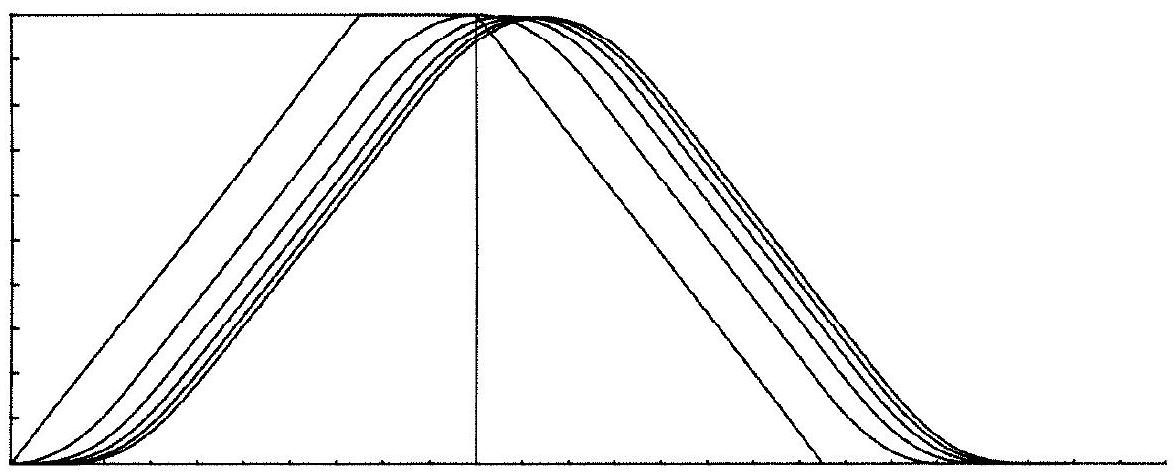
\includegraphics[max width=.8\textwidth]{2024_02_17_0c416db476dd617ef477g-007}

    Fig. 1. $u_{k}$ for $k \leqq 6$ with $a_{0}=1, a_{j}=1.5 /(j(j+1))$
\end{center}

Since $\int H_{a} d x=1$ it follows from \eqref{(1.3.4)} that
\begin{equation}
    \label{(1.3.12)'}
    \left|u_{k}^{(j)}\right| \leqq \frac{2^{j}}{a_{0} \cdots a_{j}}, \quad \int|u_{k}^{(j)}| d x \leqq \frac{2^{j}}{a_{0} \ldots a_{j-1}}
\end{equation}
for a convolution $u * v$ can always be estimated by sup $|u| \int|v| d x$. Now
\[
	\begin{aligned}
		\left|u_{k+m}-u_{m}\right| & =\left|u_{m} * H_{a_{m+1}} * \ldots * H_{a_{m+k}}-u_{m}\right|            \\
		                           & \leqq\left(a_{m+1}+\ldots+a_{m+k}\right) \sup \left|u_{m}'\right| \\
		                           & \leqq 2 a_{0}^{-1} a_{1}^{-1}\left(a_{m+1}+\ldots+a_{m+k}\right)
	\end{aligned}
\]
by the proof of \Cref{Theorem 1.3.2}, so $u_{m}$ has a uniform limit $u$. So has the derivative
\[
	u_{m}'=a_{0}^{-1}\left(1-\tau_{a_{0}}\right) H_{a_{1}} * \ldots * H_{a_{m}}
\]
and so on. By \Cref{Theorem 1.1.5} it follows that $u \in C^{\infty}$, and \eqref{(1.3.12)'} gives \eqref{(1.3.12)}. Since $\int u_{k} d x=1$ for every $k$ by \eqref{(1.3.4)}, we have $\int u d x=1$.
\end{proof}

Only in the last step was it important that $\sum a_{j}$ was assumed convergent. However, if it diverges then the limit $u$ must be identically $0$. This will follow from our next lemma which shows how precise the construction in \Cref{Theorem 1.3.5} really is.

\begin{lemma}
    If $u \in C^{m}((-\infty, T])$ vanishes on the negative half axis, and if $a_{j}$ are positive decreasing numbers with $T \leqq a_{1}+\ldots+a_{m}$, then
\begin{equation}
    \label{(1.3.13)}
    |u(x)| \leqq \sum_{j \in J} 2^{2 j} \sup _{y<x} a_{1} \ldots a_{j}\left|u^{(j)}(y)\right| \quad\text{ if }x \leqq T
\end{equation}
Here $J=\{j ; 1 \leqq j \leqq m \text{ and } a_{j+1}<a_{j} \text{ or } j=m\}$.
\end{lemma}

\begin{proof}
    The formula
\[
	u=H_{a} * a u'+\tau_{a} u
\]
used in the proof of \Cref{Theorem 1.3.5}, gives for $j \leqq m-1$ that
\begin{equation}
    \label{(1.3.14)}
    u^{(j)}=H_{a_{j+1}} * a_{j+1} u^{(j+1)}+\tau_{a_{j+1}} u^{(j)} .
\end{equation}
Starting from the case $j=0$ this allows us to write $u$ as a sum of terms of the form
\begin{equation}
    \label{(1.3.15)}
\tau_{a_{k_1}} \ldots \tau_{a_{k_i}} H_{a_1} * \ldots * H_{a_j} * a_1 \ldots a_j u^{(j)} ; \quad i \leqq m, j \leqq m, \\
\text { and } a_{k_v} \geqq a_v, \quad v \leqq i .
\end{equation}
(The last condition guarantees that $\tau_{a_{k_1}} \ldots \tau_{a_{k_{i_1}}}$ is a translation by at least $a_1+\ldots+a_i$.) We shall say that \eqref{(1.3.15)} is a legitimate term of type $(i, j)$ and represent it by the point $(i, j) \in \mathbb{R}^2$. In any term with $(i, j) \in Z$,
\[
Z=\left\{(i, j) ; 0 \leqq i<m, 0 \leqq j<m, a_{j+1} \geqq a_{i+1}\right\}
\]
we apply \eqref{(1.3.14)} and obtain two new terms. Since $a_{j+1} \geqq a_{i+1}$ the one which comes from the second term in \eqref{(1.3.14)} is legitimate of type $(i+1, j)$, and $(i+1, j) \in Z$ unless $i+1=m$, for $a_{i+2} \leqq a_{i+1}$. The other term is legitimate of type $(i, j+1)$, and we have $(i, j+1) \in Z$ unless $j+1=m$, thus $j+1 \in J$, or else $a_{j+2}<a_{i+1}$; since $a_{i+1} \leqq a_{j+1}$ this implies $i+1<j +2$ and $a_{j+2}<a_{j+1}$, hence $j+1 \in J$. After a finite number of steps we conclude that $u$ is a sum of terms of the form \eqref{(1.3.15)} with either $i \geqq m$ or $j \in J$ and $i+1 \leqq j$. (In Fig. $2(i, j)$ is a free arrowhead.) The number of terms of type $(i, j)$ is at most $2^{i+j}$ since each term corresponds to an increasing path from $(0,0)$ to $(i, j)$ among lattice points, so there are $i+j$ steps and at most two alternatives for each of them. Since
\[
	\sum_{i<j} 2^{i+j}<2^{2 j}
\]
and the terms with $i=m$ vanish in $(0, T)$, we have proved \eqref{(1.3.13)}.
\end{proof}

If we drop the assumption $T \leqq a_{1}+\ldots+a_{m}$ in Lemma 1.3.6 and set $c=T /\left(a_{1}+\ldots+a_{m}\right)$, we can apply Lemma 1.3.6 to $u(c x)$ which is defined for $x \leqq a_{1}+\ldots+a_{m}$. This gives
\begin{equation}
    \label{(1.3.13)'}
	|u(x)| \leqq \sum_{j \in J}(4 c)^{j} \sup _{y<x} a_{1} \ldots a_{j}\left|u^{(j)}(y)\right| \quad \text { if } x \leqq T
\end{equation}
If
\begin{equation}
    \label{(1.3.16)}
    \left|u^{(j)}(x)\right| \leqq \frac{K^j}{a_{1} \cdots a_{j}}\quad \text{ when } j \in J \quad \text{ and }\quad x \leqq T
\end{equation}
then it follows that
\begin{equation}
    \label{(1.3.17)}
	|u(x)| \leqq \frac{8TK}{a_{1}+\cdots+a_{m}} \quad \text { if } x \leqq T \leqq \frac{a_{1}+\cdots+a_{m}}{8 K}
\end{equation}
In fact
\[
	\sum_{1}^{\infty}(4 c K)^{j}=\frac{4cK}{1-4 c K}<8 c K \quad \text { if } 8 c K<1
\]
If we apply \eqref{(1.3.17)} to the integral of the function $u$ in \Cref{Theorem 1.3.5} taking $K=2$, we also conclude that $u$ could not have been given support in an interval shorter than $\sum a_{j} / 16$, for $8 c /(1-8 c)<1$ if $c<1 / 16$. Apart from a fixed scale factor the construction in \Cref{Theorem 1.3.5} is therefore quite precise. If $\sum a_{j}=\infty$ and \eqref{(1.3.16)} is valid for all $j$ we may also conclude that $u \equiv 0$. In fact, we shall deduce the complete \hyperref[thm:1.3.8]{Denjoy--Carleman theorem}.

Let $M_{0}=1, M_{1}, M_{2}, \ldots$ be a sequence of positive numbers, and denote by $C^{M}([a, b])$ the set of all $u \in C^{\infty}([a, b])$ such that for some $K$
\begin{equation}
    \label{(1.3.18)}
    \left|u^{(j)}(x)\right| \leqq K^{j+1} M_{j} \quad \text{ if } a \leqq x \leqq b \quad \text{ and }j=0,1, \ldots
\end{equation}
\begin{defi}
    $C^{M}$ is called quasi-analytic if $u^{(j)}(x)=0$ for every $j$ at some $x \in[a, b]$ implies $u=0$ in $[a, b]$ when $u \in C^{M}([a, b])$.
\end{defi}
Let
\begin{equation}
    \label{1.3.19}
	L_{j}=\inf _{k \geqq j} M_{k}^{1 / k}
\end{equation}
be the largest increasing minorant of $M_{k}^{1 / k}$ and let $M_{j}^{*}$ be the largest logarithmically convex minorant of the sequence $M_{j}$,
\begin{equation}
    \label{(1.3.20)}
    M_{j}^{*}=\inf \left\{M_{j}, M_{k}^{(l-j) /(l-k)} M_{l}^{(j-k) /(l-k)}\right. \text{ when } \left.k<j<l\right\}.
\end{equation}
Thus $M_{j}^{* 2} \leqq M_{j-1}^{*} M_{j+1}^{*}, j>0$, which shows that $M_{j}^{*}>0$ for all $j$ unless $M_{j}^{*}=0$ for every $j>0$. Moreover,
\begin{equation}
    \label{(1.3.21)}
    a_{j}= \frac{M_{j-1}^{*}}{M_{j}^{*}}, \quad j=1,2, \ldots
\end{equation}
is a decreasing sequence. (We define $a_{j}=+\infty$ if $M_{j}^{*}=0$.)

\begin{theorem}[Denjoy--Carleman]
    The following conditions are equivalent:
\begin{enumerate}
    \item $C^{M}$ is quasi-analytic.
    \item $\sum_{0}^{\infty} 1 / L_{j}=\infty$.
    \item  $\sum_{0}^{\infty}\left(M_{j}^{*}\right)^{-1 / j}=\infty$.
    \item $\sum_{1}^{\infty} a_{j}-\infty$.
\end{enumerate}
\end{theorem}
\begin{proof}
    First we consider the rather uninteresting case where $L_{j} \leqq L<\infty$ for every $j$, that is, $\lim M_{k_{j}}^{1 / k_{j}} \leqq L$ for some sequence $k_{j} \rightarrow \infty$. Letting $l$ run through this sequence in \eqref{(1.3.20)} and taking $k=0$ there we obtain
\[
	L^{j} M_{0} \geqq M_{j}^{*}= \frac{M_{0}}{a_{1} \ldots a_{j}}  \geqq \frac{M_{0}}{a_{1} \ldots a_{i-1} a_{i}^{i-j-1}}, \quad i \leqq j
\]
and this implies $a_{i}^{-1} \leqq L$. Thus the conditions (ii), (iii), (iv) are fulfilled. If $u$ satisfies (1.3.18) and $u^{(j)}(x_0)=0$ for every $j$, then Taylor's formula gives for every $x \in[a, b]$
\[
	|u(x)| \leqq \frac{K^{k_{j}+1}\left|x-x_{0}\right|^{k_{j}} M_{k_{j}}}{k_{j} !} \rightarrow 0 \quad \text { when } j \rightarrow \infty.
\]
Thus (i) is also valid.

Assume now that $L_{j} \rightarrow \infty$ when $j \rightarrow \infty$, that is, that $M_{k}^{1 / k} \rightarrow \infty$ as $k \rightarrow \infty$. Then the points $\left(k, \log M_{k}\right)$ will lie above lines with arbitrarily high slope so $M_{j}^{*}$ is positive and $a_{j} \rightarrow 0$. Thus $\hat{J}=\left\{j ; a_{j+1}<a_{j}\right\}$ is an infinite set where the graph of $\log M_{k}^{*}$ as a function of $k$ has a corner. This implies that $M_{j}^{*}=M_{j}$ when $j \in \hat{J}$; analytically this follows since for $k<j<l$
\[
	\begin{aligned}
		 & M_{k}^{(l-j) /(l-k)} M_{l}^{(j-k) /(l-k)} \geqq M_{k}^{*(l-j) /(l-k)} M_{l}^{*(j-k) /(l-k)}                                                      \\
		 & \quad \geqq M_{j}^{*} a_{j}^{(l-j)(j-k) /(l-k)} a_{j+1}^{-(l-j)(j-k) /(l-k)} \geqq M_{j}^{*}\left(\frac{a_{j}}{a_{j+1}}\right)^{\frac{1}{2}}>M_{j}^{*}
	\end{aligned}
\]
Since
\[
	M_{k}^{*}= \frac{M_{0}^{*}}{a_{1} \cdots a_{k}}  \leqq a_{k}^{-k}
\]
it follows that $M_{j}^{1 / j} \leqq 1 / a_{j}$ when $j \in \widehat{J}$. If $k<j \in \widehat{J}$ and $k \leqq i<j$ implies $i \notin \hat{J}$ then $a_{i}=a_{j}$ for $k \leqq i \leqq j$ so it follows that $L_{i} \leqq L_{j} \leqq 1 / a_{j}=1 / a_{i}$, hence
$L_{j} \leqq 1 / a_{j}$ for every $j$. This proves that (iv) $\Rightarrow$ (ii). Since $\log M_{j}^{*}$ is a convex function of $j$ and vanishes when $j=0$ the slope $j^{-1} \log M_{j}^{*}$ of the chord from $(0,0)$ is increasing, that is, $\left(M_{j}^{*}\right)^{1 / j}$ is increasing. Hence $L_{j} \geq\left(M_{j}^{*}\right)^{1 / j}$ which proves that (ii) $\Rightarrow$ (iii). If (iv) is false we know from \Cref{Theorem 1.3.5} that there is a function $u \neq 0$ in $C_{0}^{\infty}([a, b])$ with
\[
	\left|u^{(j)}(x)\right| \leqq \frac{K^{j+1}}{a_{1} \cdots a_{j}} =K^{j+1} M_{j}^{*} \leqq K^{j+1} M_{j}
\]
so (i) is not valid. Thus (i) $\Rightarrow$ (iv). On the other hand, if (iv) is valid we can apply \eqref{(1.3.17)} with $m$ equal to an element of $\hat{J}$. The set $J$ in \eqref{(1.3.16)}, defined in Lemma 1.3.6, is then the set of elements $\leqq m$ in $\hat{J}$, so \eqref{(1.3.16)} follows from \eqref{(1.3.18)} since $M_{j}=M_{j}^{*}=1 / a_{1} \ldots a_{j}$ when $j \in \hat{J}$. Hence (iv) $\Rightarrow$ (i). The remaining proof that (iii) $\Rightarrow$ (iv) follows from

\begin{lemma}[Carleman's inequality]
    If $a_{j}>0$ then
\begin{equation}
    \label{(1.3.22)}
	\sum_{1}^{\infty}\left(a_{1} a_{2} \ldots a_{n}\right)^{1 / n} \leqq e \sum_{1}^{\infty} a_{n} 
\end{equation}
\end{lemma}
\begin{proof}
    With $c_{j}$ to be chosen later we have by the inequality between geometric and arithmetic means
\[
	\left(a_{1} \ldots a_{n}\right)^{1 / n}=\left(c_{1} \ldots c_{n}\right)^{-1 / n}\left(c_{1} a_{1} \ldots c_{n} a_{n}\right)^{1 / n} \leqq\left(c_{1} \ldots c_{n}\right)^{-1 / n} n^{-1} \sum_{1}^{n} c_{m} a_{m}
\]
If we choose $c_{m}=(m+1)^{m} / m^{m-1}$ then $\left(c_{1} \ldots c_{n}\right)^{1 / n}=n+1$ and we have
\[
	\sum\left(a_{1} \ldots a_{n}\right)^{1 / n} \leqq \sum_{1 \leqq m \leqq n} \frac{c_{m} a_{m}}{n(n+1)}=\sum_{1}^{\infty} \frac{c_{m} a_{m}}{m} \leqq \sum_{1}^{\infty} e a_{m}
\]
which proves \eqref{(1.3.22)}.

When $M_{n}=n!$ then Taylor's formula gives for $f \in C^{M}([a, b])$ that
\[
	f(x)=\sum_{0}^{\infty} \frac{f^{(j)}(y)(x-y)^{j}}{j!}
\]
if $x, y \in[a, b]$ and $|x-y|<r$. Thus \Cref{Theorem 1.3.8} is completely elementary in this case. Note that the Taylor series is then absolutely convergent for all $x \in \mathbb{C}$ with $|x-y|<r$ and it gives an analytic continuation of $f$ to
\[
	\{z \in \mathbb{C} ;|z-y|<r \text { for some } y \in[a, b]\}
\]
Conversely, if $F$ is an analytic function in a complex neighborhood of $[a, b]$ then the restriction of $F$ to $[a, b]$ is in $C^{M}([a, b])$ by Cauchy's inequalities. Accordingly this class is called the class of real analytic functions. It is obvious that the preceding remarks can be applied also to functions of several variables.
\qedhere\qedsymbol\end{proof}\def\qedsymbol{}
\end{proof}

\section{Cutoff Functions and Partitions of Unity}
In distribution theory one often has to replace a function by one with compact support without changing it on a large compact set. This is done by multiplication with a "cutoff function" as constructed in the following
\begin{theorem}
    If $X$ is an open set in $\mathbb{R}^{n}$ and $K$ is a compact subset, then one can find $\phi \in C_{0}^{\infty}(X)$ with $0 \leqq \phi \leqq 1$ so that $\phi=1$ in a neighborhood of $K$.
\end{theorem}
\begin{proof}
    Choose $\varepsilon>0$ so small that
\begin{equation}
    \label{(1.4.1)}
	|x-y| \geqq 4 \varepsilon \quad \text { when } \quad x \in K, y \in\complement X
\end{equation}
and let $v$ be the characteristic function of
\[
	K_{2 \varepsilon}=\{y ;|x - y| \leqq 2 \varepsilon \text { for some } x \in K\}
\]
According to \Cref{Lemma 1.2.3} we can find a non-negative function $\chi \in C_{0}^{\infty}(B)$ where $B$ is the unit ball, such that $\int \chi d x=1$. Then $\chi_{\varepsilon}(x)=\varepsilon^{-n} \chi(x / \varepsilon)$ has support in the ball $\{x ;|x|<\varepsilon\}$ and $\int \chi_{\varepsilon} d x=1$, so
\[
	\phi=v * \chi_{\varepsilon} \in C_{0}^{\infty}\left(K_{3 \varepsilon}\right)
\]
by \Cref{Theorem 1.3.1} and \eqref{(1.3.11)}, and $1-\phi=(1-v) * \chi_{\varepsilon}$ vanishes in $K_{\varepsilon}$ by \eqref{(1.3.11)}. This proves the theorem.
\end{proof}

For future reference we also note that
\[
	\left|\partial^{\alpha} \phi\right| \leqq \int\left|\partial^{\alpha} \chi_{\varepsilon}\right| d x=\varepsilon^{-|\alpha|} \int\left|\partial^{\alpha} \chi\right| d x .
\]
Thus
\begin{equation}
    \label{(1.4.2)}
    \left|\partial^{\alpha} \phi\right| \leqq C_{\alpha} \varepsilon^{-|\alpha|}
\end{equation}
where $C_{\alpha}$ only depends on $\alpha, n$ and the choice of the norm. Using \Cref{Theorem 1.3.5} it is possible to give a still more precise result which we mention for the sake of completeness since it is sometimes useful. However, the reader can jump to \Cref{Theorem 1.4.4} without loss of continuity.
\begin{theorem}
    Let $X$ be an open set in the $n$ dimensional vector space $V$ with norm $\|\cdot\|$ and let $K$ be a compact subset. If
\[
d = \inf\{\|x-y\|; x\in \complement X,y\in K\}
\]
and $d_{j}$ is a positive decreasing sequence with $\sum_{1}^{\infty} d_{j}<d$, then one can find $\phi \in C_{0}^{\infty}(X)$ with $0 \leqq \phi \leqq 1$, equal to 1 in a neighborhood of $K$, so that
\begin{equation}
    \label{(1.4.3)}
    \left|\phi^{(k)}\left(x ; y_{1}, \ldots, y_{k}\right)\right| \leqq \frac{C^{k}\left\|y_{1}\right\| \ldots\left\|y_{k}\right\|}{d_{1} \ldots d_{k}} ; \quad k=1,2, \ldots
\end{equation}
Here $C$ depends only on the dimension $n$.
\end{theorem}
\begin{proof}
    Assume first that $V=\mathbb{R}^{n}$ and that $\|x\|=\max \left|x_{j}\right|$. Let $u$ be the function in \Cref{Theorem 1.3.5} with $a_{j}=d_{j+1}$ and set $h(t)=u\left(t+\sum d_{j} / 2\right)$. Then we have $|t| \leqq \sum\left|d_{j}\right| / 2$ if $t \in \operatorname{supp} h$, and for every $j$
\[
	\int\left|h^{(j)}(t)\right| d t \leqq 2^{j} / d_{1} \ldots d_{j}, \quad \int h(t) d t=1
\]
We can now apply the proof of \Cref{Theorem 1.4.1} with $\varepsilon=1$ and
\[
	\chi(x)=h\left(x_{1}\right) \ldots h\left(x_{n}\right)
\]
taking for $v$ the characteristic function of
\[
	\{y ;\|x-y\| \leqq d / 2 \text { for some } x \in K\}
\]
It follows that
\[
	\left|\partial^{\alpha} \phi\right| \leqq \int\left|\partial^{\alpha} \chi\right| d x \leqq 2^{|\alpha|} / d_{1} \ldots d_{|\alpha|}
\]
so introducing the differentials instead we have
\[
	\left|\phi^{(k)}\left(x ; y_{1}, \ldots, y_{k}\right)\right| \leqq(2 n)^{k}\left\|y_{1}\right\| \ldots\left\|y_{k}\right\| / d_{1} \ldots d_{k}
\]
which proves \Cref{THeorem 1.4.2} in this case. The passage to a Euclidean norm and from there to an arbitrary norm can be made by the following lemma which gives \eqref{(1.4.3)} with $C=2 n^{2}$.
\end{proof}
\begin{lemma}
    If $K$ is a convex symmetric body in the $n$ dimensional vector space $V$, then one can find an ellipsoid $B$ with center at $0$ and
\[
	B \subset K \subset B \sqrt{n}
\]
\end{lemma}
\begin{proof}
    Proof. Let $B$ be an ellipsoid of maximal volume contained in $K$ and choose coordinates so that $B$ is the unit ball. We have to show that $K\subset B \sqrt{n}$. To do so we assume that $K$ contains a point $(t, 0, \ldots, 0)$ with $t>\sqrt{n}$ and prove that $B$ cannot be maximal then. The tangent cone to $B$ with vertex at $(t, 0, \ldots, 0)$ touches $B$ where $x_{1}=1 / t$, so the part of $B$ where $\left|x_{1}\right|>1 / t$ is in the interior of $K$ because of the convexity and symmetry with respect to 0 . Now consider the ellipsoid
\[
	(1-\varepsilon)^{n-1} x_{1}^{2}+ \frac{y^{2}}{1-\varepsilon}\leqq 1, \quad y=\left(x_{2}^{2}+\ldots+x_{n}^{2}\right)^{\frac{1}{2}}
\]
which has the same volume as $B$. The inequality may be written
\[
    x_{1}^{2}+y^{2}-\left((n-1) x_{1}^{2}-y^{2}\right) \varepsilon+O\left(\varepsilon^{2}\right)<1     
\]
that is
\[
    \left(x_{1}^{2}+y^{2}-1\right)(1+\varepsilon)<\varepsilon\left(n x_{1}^{2}-1\right)+O\left(\varepsilon^{2}\right)
\]
\begin{center}
	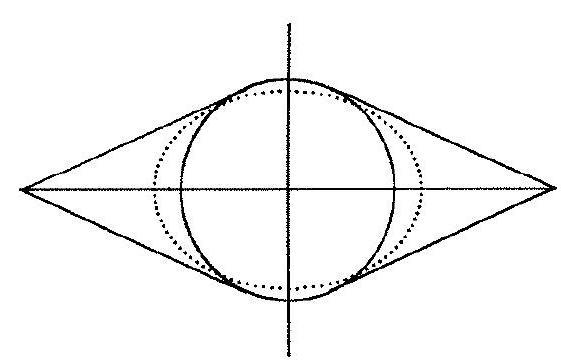
\includegraphics[max width=.5\textwidth]{2024_02_17_0c416db476dd617ef477g-009(1)}
    
    Fig. 3
\end{center}
For small $\varepsilon>0$ the right-hand side is negative when $\left|x_{1}\right|<(1 / t+1 / \sqrt{n}) / 2$ so this part of the ellipsoid is in the interior of $K$. But this is also true of the remaining part since $\left|x_{1}\right| \geqq(1 / t+1 / \sqrt{n}) / 2>1 / t$. (See Fig. 3.) Hence $B$ is not maximal.
\end{proof}


An equivalent way of stating \Cref{Lemma 1.4.3} is of course that for any norm $\|\cdot \|$ in $V$ one can find a Euclidean norm $\|\cdot\|$ such that
\[
	|x| \leqq\|x\| \leqq|x| \sqrt{n}, \quad x \in V
\]
In order to make conclusions about a distribution from local hypotheses, it is necessary to write arbitrary test functions as sums of test functions of small support.
\begin{theorem}
    Let $X_{1}, \ldots, X_{k}$ be open sets in $\mathbb{R}^{n}$ and let $\phi \in C_{0}^{\infty}\left(\bigcup_{1}^{k} X_{j}\right)$. Then one can find $\phi_{j} \in C_{0}^{\infty}\left(X_{j}\right), j=1, \ldots, k$, such that
\begin{equation}
    \label{(1.4.4)}
	\phi=\sum_{1}^{k} \phi_{j}
\end{equation}
If $\phi \geqq 0$ one can take all $\phi_{j} \geqq 0$.
\end{theorem}
\begin{proof}
    We can choose compact sets $K_{1}, \ldots, K_{k}$ with $K_{j} \subset X_{j}$ so that $\operatorname{supp} \phi \subset \bigcup_{1}^{k} K_{j}$. (In fact, every point in supp $\phi$ has a compact neighborhood contained in some $X_{j}$. By the Borcl-Lebesgue lemma a finite number of such neighborhoods can be chosen which cover all of supp $\phi$. The union of those which belong to $X_{j}$ is a compact set $K_{j}\subset X_{j}$.) Using Theorem 1.4 .1 we now choose $\psi_{j} \in C_{0}^{\infty}\left(X_{j}\right)$ with $0 \leqq \psi_{j} \leqq 1$ and $\psi_{j}=1$ in $K_{j}$. Then the functions
\[
	\phi_{1}=\phi \psi_{1}, \phi_{2}=\phi \psi_{2}\left(1-\psi_{1}\right), \ldots, \phi_{k}=\phi \psi_{k}\left(1-\psi_{1}\right) \ldots\left(1-\psi_{k-1}\right)
\]
have the required properties since
\[
	\sum_{1}^{k} \phi_{j}-\phi=-\phi \prod_{1}^{k}\left(1-\psi_{j}\right)=0
\]
because either $\phi$ or some $1-\psi_{j}$ is zero at any point.
\end{proof}

Combining Theorems 1.4.4 and 1.4.1 we obtain
\begin{theorem}
    Let $X_{1}, \ldots, X_{k}$ be open sets in $\mathbb{R}^{n}$ and $K$ a compact
    subset of $\bigcup_1^k X_j$. Then one can find $\phi_j \in C_0^{\infty}\left(X_j\right)$ so that $\phi_j \geqq 0$ and
$\sum_{1}^{k} \phi_{j} \leqq 1$ with equality in a neighborhood of $K$.
\end{theorem}
\begin{remark}
    In Theorems 1.4.4 and 1.4.5 we could allow an infinite number of open sets $X_{j}$ while in the conclusion only finitely many $\phi_{j}$ are not identically 0 . In fact, by the Borel-Lebesgue lemma a finite number of the sets $X_{j}$ suffice to cover supp $\phi$ and $K$ respectively.

The functions $\phi_{j}$ in \Cref{Theorem 1.4.5} are said to be a partition of unity at $K$ subordinate to the covering of $K$ by the sets $X_{j}$. Infinite partitions of unity are sometimes required, and for the sake of completeness we shall give one simple and one fairly intricate example.
\end{remark}
\begin{theorem}
    For every neighborhood $X$ of the cube
\[
	K=\left\{x \in \mathbb{R}^{n} ;\left|x_{j}\right| \leqq \frac{1}{2}, j=1, \ldots, n\right\}
\]
one can find a non-negative function $\phi \in C_{0}^{\infty}(X)$ such that
\[
	\sum \phi(x-g)=1
\]
where $g$ runs over all lattice points, that is, points with integer coordinates.
\end{theorem}
\begin{proof}
    By \Cref{Theorem 1.4.1} we can choose $\psi \in C_{0}^{\infty}(X)$ so that $0 \leqq \psi \leqq 1$ and $\psi=1$ on $K$. Hence
\[
	\Psi(x)=\sum \psi(x-g)
\]
is a periodic $C^{\infty}$ function with $\Psi(x) \geqq 1$ everywhere, so $\phi(x)=\psi(x) / \Psi(x)$ has the required properties.

\Cref{Theorem 1.4.6} gives a partition of unity subordinate to the covering of $\mathbb{R}^{n}$ by the translates $X+\{g\}$ of $X$. Wc shall now construct partitions of unity corresponding to a covering by convex symmetric neighborhoods which may vary both in size and in shape. It is convenient to describe the neighborhoods in terms of the corresponding norms.
\end{proof}

\begin{defi}
    If $X$ is an open set in a finite dimensional vector space $V$ and $\|\cdot \|_{x}$ for every $x \in X$ is a norm in $V$, then we shall say that we have a slowly varying metric in $X$ if
\begin{equation}
    \label{(1.4.5)}
    x \in X, \quad\|y-x\|_{x}<1 \text{ implies } y \in X \text{ and } \|v\|_{y} \leqq C\|v\|_{x}, \quad v \in V
\end{equation}
where $C \geqq 1$ is independent of $x, y, v$.
\end{defi}

Note that if $C\|x-y\|_{x}<1$ then $\|x-y\|_{y}<1$ so
\[
	\|v\|_{x} \leqq C\|v\|_{y}, \quad v \in V
\]
Replacing the norm ||$_{x}$ by $C\|\|_{x}$ we have therefore
\begin{equation}
    \label{(1.4.5)'}
    C^{-1}\|v\|_{x} \leqq\|v\|_{y} \leqq C\|v\|_{x} \quad \text { if }\|x-y\|_{x}<1
\end{equation}
which we shall assume from now on.

\begin{example}
    Let $X$ be an open set in $V$ and $d(x)$ a Lipschitz continuous function, positive in $X$ and zero in $V \setminus X$, with
\[
	|d(x)-d(y)| \leqq\|x-y\| \quad \text { if } x, y \in X
\]
where $\|\cdot \|$ is a fixed norm in $V$. Then
\[
	\|v\|_{x}= \frac{2\|v\|}{d(x)}
\]
defines a slowly varying metric in $X$, for $\|x-y\|_{x}<1$ means that $\|x-y\|<d(x) / 2$ which implies $|d(x)-d(y)|<d(x) / 2$ and $d(x) / 2<d(y)<2 d(x)$. For any given open set $X \neq V$ we may always take for $d(x)$ the distance to $F=\complement X$ defined by
\[
	d(x)=\inf _{y \in F}\|x-y\|
\]
We shall now show how a slowly varying metric gives rise first to a covering and then to a subordinate partition of unity.
\end{example}
\begin{lemma}
    Let $\varepsilon<1 / C$ and choose a maximal sequence $x_{1}, x_{2}, \ldots$ in $X$ such that
\begin{equation}
    \label{(1.4.6)}
	\left\|x_{\mu}-x_{v}\right\|_{r_{v}} \geqq \varepsilon \quad \text { when } v \neq \mu.
\end{equation}
Then the balls
\[
	B_{v}^{R}=\left\{x ;\left\|x-x_{v}\right\|_{x_{v}}<R\right\}
\]
where $\varepsilon C<R<1$, are a covering of $X$, and no point belongs to more than $N=\left(2 C^{2} / \varepsilon+1\right)^{n}$ different $B_{v}^{R}$.
\end{lemma}
\begin{proof}
    The existence of a maximal sequence follows from the fact that a set satisfying (1.4.6) is necessarily discrete. If $x \in X$ cannot be added to the sequence then either $\left\|x-x_{v}\right\|_{x_{v}}<\varepsilon$ or else $\left\|x-x_{v}\right\|_{x}<\varepsilon$ for some $v$, and in the latter case it follows that $\left\|x-x_{v}\right\|_{\Lambda_{v}}<C$ s so $x \in B_{v}^{R}$ in any case. If $x \in B_{v}^{R}$ we obtain since $R<1$
\[
	\left\|x-x_{v}\right\|_{x}<C
\]
and if $x \in B_{u}^{R}$ also then
\[
	\varepsilon \leqq\left\|x_{\mu}-x_{v}\right\|_{x_{v}} \leqq C\left\|x_{\mu}-x_{v}\right\|_{x}
\]
Hence the balls
\[
	\left\{y ;\left\|y-x_{v}\right\|_{x}< \frac{\varepsilon}{2C}\right\}
\]
are disjoint when $x \in B_{v}^{R}$, and they are all contained in the ball
\[
	\left\{y ;\|x-y\|_{x}<C+\frac{\varepsilon}{2C}\right\}
\]
so the number of such $v$ cannot exceed the ratio $\left(2 C^{2} / \varepsilon+1\right)^{n}$ of the measures.
\end{proof}

Choose $\varepsilon=1 / 2 C$ and for every $v$ a non-negative function $\psi_{v} \in C_{0}^{\infty}\left(B_{v}^{1}\right)$ which is $1$ in $B_{v}^{\frac{1}{2}}$ and for a given decreasing sequence $d_{j}$ with $\sum d_{j}=1$ has the estimate
\[
	\left|\psi_{v}^{(k)}\left(x ; y_{1}, \ldots, y_{k}\right)\right| \leqq \frac{C_{1}^{k}\left\|y_{1}\right\|_{x_{v}} \ldots\left\|y_{k}\right\|_{x_{v}}}{d_{1} \ldots d_{k}}
\]
This is possible by \Cref{Theorem 1.4.2} with $C_{1}$ equal to three times the constant in \eqref{(1.4.3)}. Since $\|y\|_{x_{\nu}} \leqq C\|y\|_{x}$ for every $x \in \operatorname{supp} \psi_{v}$ we obtain
\[
	\left|\psi_{v}^{(k)}\left(x ; y_{1}, \ldots, y_{k}\right)\right| \leqq \frac{\left(C C_{1}\right)^{k}\left\|y_{1}\right\|_{x} \ldots\left\|y_{k}\right\|_{x}}{d_{1} \ldots d_{k}}
\]
As in the proof of \Cref{Theorem 1.4.4} we now introduce
\[
	\phi_{v}=\psi_{v}\left(1-\psi_{1}\right) \ldots\left(1-\psi_{v-1}\right)
\]
and obtain $\sum \phi_{\nu}=1$ in $X$. No point is in the support of more than $N$ factors $\psi_{\mu}$. Now note that if for some norm we have at $x$
\[
	\left|f_{j}^{(k)}\left(x, y_{1}, \ldots, y_{k}\right)\right| \leqq \frac{A_{j}^{k}\| y_{1}\|\ldots\| y_{k} \|}{d_{1} \ldots d_{k}}
\]
for $k=0,1, \ldots$ and $j=1,2$, then the same estimate is valid for $f_{1} f_{2}$ with the constant $A_{1}+A_{2}$ instead. This follows from the fact that $d_{j}$ is decreasing and from the rules for differentiating a product. Hence
\[
	\left|\phi_{v}^{(k)}\left(x ; y_{1}, \ldots, y_{k}\right)\right| \leqq\frac{\left(N C C_{1}\right)^{k}\|y_{1}\|_{x} \ldots\| y_{k} \|_{x}}{d_{1} \ldots d_{k}}
\]
We have now proved
\begin{theorem}
    For any slowly varying metric in the open set $X$ in the $n$ dimensional vector space $V$ one can choose a sequence $x_{v} \in X$ such that the balls
\[
	B_{v}=\left\{x ;\left\|x-x_{v}\right\|_{x_{v}}<1\right\}
\]
form a covering of $X$ for which the intersection of more than $N=\left(4 C^{3}\right.+1)^{n}$ balls $B_{v}$ is always empty. Moreover, for any decreasing sequence $d_{j}$ with $\sum d_{j}=1$ one can choose non-negative $\phi_{v} \in C_{0}^{\infty}\left(B_{v}\right)$ with $\sum \phi_{v}=1$ in $X$ so that for all $k$
\begin{equation}
    \label{(1.4.7)}
	\left|\phi_{v}^{(k)}\left(x ; y_{1}, \ldots, y_{k}\right)\right| \leqq\frac{\left(N C C_{1}\right)^{k}\|y_{1}\|_{x} \ldots\| y_{k} \|_{x}}{d_{1} \ldots d_{k}}
\end{equation}
where $C$ is the constant in \eqref{(1.4.5)} and $C_{1} / 3$ is that in \eqref{(1.4.3)} so it only depends on $n$.
\end{theorem}
\begin{remark}
    Without changing the proof one may allow $d_{j}$ to be functions of $x$ provided that they vary slowly with respect to the metric, that is
    \begin{equation}
        \label{(1.4.5)'} 
        d_{j}(y) \leqq C d_{j}(x) \text{ if } x \in X \text{ and } \|y-x\|_{x}<1
    \end{equation}
\end{remark}
The following corollary is sometimes a useful supplement to \Cref{Theorem 1.4.1}.
\begin{cor}
    Let $F_{0}$ and $F_{1}$ be two closed sets in $\mathbb{R}^{n}$. Then one can find $\phi \in C^{\infty}\left(\complement\left(F_{0} \cap F_{1}\right)\right)$ such that $\phi=0$ near $F_{0} \setminus\left(F_{0} \cap F_{1}\right), \phi=1$ near $F_{1} \setminus\left(F_{0} \cap F_{1}\right)$ and, with the notation in \Cref{Theorem 1.4.10},
Here
\begin{equation}
    \label{(1.4.8)}
	\left|\phi^{(k)}\left(x ; y_{1}, \ldots, y_{k}\right)\right| \leqq \frac{C_{2}^{k}\left\|y_{1}\right\| \ldots\left\|y_{k}\right\| d(x)^{-k}}{d_{1} \ldots d_{k}} 
\end{equation}
\[
	d(x)=\max \left(d\left(x, F_{0}\right), d\left(x, F_{1}\right)\right), \quad d\left(x, F_{j}\right)=\min _{y \in F_{j}}\|x-y\| .
\]
The support of $\phi$ is bounded if $F_{1}$ is compact.
\end{cor}
\begin{proof}
    $d(x)$ is Lipschitz continuous with Lipschitz constant 1 , so $\|v\|_{x}=2\|v\| / d(x)$ is a slowly varying metric in $\complement\left(F_{0} \cap F_{1}\right)$ (\Cref{Example 1.4.8}). A ball
\begin{equation}
    \label{(1.4.9)}
	\left\{y ;\|x-y\|_{x} \leqq 1\right\} 
\end{equation}
cannot meet both $F_{0}$ and $F_{1}$, for if $d(x)=d\left(x, F_{j}\right)$ then $\|x-y\|\leqq d\left(x, F_{j}\right) / 2$, hence $d\left(y, F_{j}\right) \geqq d\left(x, F_{j}\right) / 2$ in the ball. If we form the partition of unity in \Cref{Theorem 1.4.10} we can therefore take $\phi$ equal to the sum of all $\phi_{v}$ with support meeting $F_{1}$. If $F_{1}$ is compact then $d\left(x, F_{0}\right)<2 d\left(x, F_{1}\right)$ when $|x|$ is large enough. Thus $d(x)<2 d\left(x, F_{1}\right)$ so \eqref{(1.4.9)} cannot meet $F_{1}$ then. Hence supp $\phi$ will be bounded.
\end{proof}

\section{Notes}
As pointed out in the summary the introductory Section 1.1 contains only classical material and we shall not discuss its history. The test functions used in Section 1.2 also have a long tradition in the calculus of variations. Thus Theorem 1.2.4 is very close to the de Bois Reymond lemma found in all introductory texts on this topic. Theorem 1.2.6 is due to Borel [1]. More refined extension theorems are given later as Corollary 1.3.4 and Theorem 2.3.6.

The construction of infinitely differentiable functions by means of repeated convolutions used in the proof of \Cref{Theorem 1.3.5} has ancient

roots in harmonic analysis. It was used explicitly and systematically by Mandelbrojt [1,2] who attributes the idea to unpublished work by H.E. Bray. The method reappeared in the work by Ehrenpreis [3] on convolution operators and has been used frequently in the theory of partial differential equations since then (cf. Hörmander [21, 27, 30]). Cohen [2] observed that the proof by Bang [1] of the DenjoyCarleman theorem can be phrased in similar terms. We use a variant of his approach combined with arguments from Mandelbrojt [2] in our proof. Quasi-analyticity will play a role in Section 8.4. Perhaps it is appropriate to mention here that the problem of characterizing quasi-analytic classes originates from the theory of partial differential equations (see Hadamard [1, p. 37]).

Continuous partitions of unity on compact sets were defined by Dieudonné [1], and the term Dieudonné decomposition was actually current for a while. The construction in the proof of Theorem 1.4.4 is taken from the third edition of the classical monograph on Riemann surfaces by Weyl [2] where the main change was actually the use of partitions of unity. However, the covering lemma 1.4.9 and the partition of unity in Theorem 1.4.10 are essentially from Whitney [1] which shows that very sophisticated partitions of unity were used several years before Dieudonné's note. Whitney's lemma occurs in the original form as Lemma 2.3.7 below. A more general version was stated by Treves [5]. The full generality given in Section 1.4 is needed in the general theory of pseudo-differential operators (Chapter XVIII). The combination of these ideas with the repeated convolutions of Section 1.3 is probably new in its full generality but special cases can be found for example in Andersson [1].
